\chapter{Release 1 : Socle technique, authentification et planification locale}
\label{chap:release1}


\section*{Introduction}

Ce troisième chapitre présente la réalisation de la \textbf{Release 1}, regroupant le \textbf{Sprint 1} (socle technique, authentification sécurisée JWT, gestion du référentiel des sites industriels et supervision d'administration) et le \textbf{Sprint 2} (planification locale des Équipements, des Espaces et des Ressources Humaines avec moteur d'importation Excel).

\section{Sprint 1 : Socle technique, authentification et administration des sites}

\subsection{Objectifs du sprint 1}
Le Sprint 1 visait deux objectifs fondamentaux :
\begin{enumerate}
    \item Instancier l'architecture logicielle 3-tiers (Node.js/Express, React, Microsoft SQL Server \texttt{GALIA\_V1} via Sequelize) et le modèle de sécurité.
    \item Sécuriser l'accès au portail via JWT HttpOnly et doter l'Administrateur des outils de gestion du référentiel des 10 sites industriels et du tableau de bord de supervision.
\end{enumerate}

\subsection{Backlog du sprint 1}
Le Tableau \ref{tab:backlog_sprint1} présente le backlog détaillé du Sprint 1 dédié au socle technique, à l'authentification et à la gestion des sites industriels.

\begin{table}[H]
\centering
\begin{tabular}{|c|p{9.2cm}|c|c|}
\hline
\textbf{Id} & \textbf{Fonctionnalités (User Story)} & \textbf{Priorité} & \textbf{Estimation (Jours)} \\ \hline
1 & En tant qu'utilisateur, je veux accéder à une interface de connexion épurée pour saisir mes identifiants. & 1 & 1 \\ \hline
2 & En tant qu'utilisateur, je veux m'authentifier via mon email et mon mot de passe afin d'accéder au système. & 1 & 2 \\ \hline
3 & En tant qu'utilisateur, je veux que mes mots de passe soient hachés avec l'algorithme Bcrypt pour garantir leur confidentialité. & 1 & 2 \\ \hline
4 & En tant qu'utilisateur, je veux bénéficier d'un cookie sécurisé HttpOnly contenant le jeton JWT pour maintenir ma session. & 1 & 3 \\ \hline
5 & En tant qu'utilisateur, je veux me déconnecter en toute sécurité avec destruction du cookie de session et redirection. & 1 & 1 \\ \hline
6 & En tant qu'utilisateur, je veux que le système vérifie mes droits RBAC sur chaque route protégée pour bloquer les accès illégitimes. & 1 & 3 \\ \hline
7 & En tant qu'utilisateur, je veux disposer d'un menu de navigation responsive (Home Page) affichant les modules autorisés. & 1 & 2 \\ \hline
8 & En tant qu'Administrateur, je veux consulter la liste des 10 sites industriels mondiaux de COFAT avec leurs caractéristiques. & 1 & 3 \\ \hline
9 & En tant qu'Administrateur, je veux administrer et configurer le référentiel des sites de production COFAT. & 1 & 3 \\ \hline
10 & En tant qu'utilisateur, je veux sélectionner un site actif parmi le référentiel industriel pour charger ses planifications spécifiques. & 1 & 2 \\ \hline
11 & En tant qu'Administrateur, je veux consulter un tableau de bord d'administration pour superviser l'état global du parc applicatif. & 2 & 3 \\ \hline
\end{tabular}
\caption{Backlog du Sprint 1}
\label{tab:backlog_sprint1}
\end{table}

\subsection{Technologies utilisées}
La sélection de la \textit{stack} technique repose sur une approche \textit{Full-Stack JavaScript} couplée au SGBD relationnel d'entreprise Microsoft SQL Server :
\begin{itemize}
    \item \textbf{Backend :} Node.js et Express.js pour l'API RESTful (port 9001), avec \texttt{jsonwebtoken} pour la signature des jetons, \texttt{bcryptjs} pour le hachage des mots de passe, \texttt{cookie-parser} et \texttt{multer} pour la gestion des fichiers.
    \item \textbf{Base de données \& ORM :} Microsoft SQL Server (instance \texttt{GALIA\_V1}, port 1433) manipulée via l'ORM Sequelize (v6) pour la persistance relationnelle et la protection native contre les injections SQL.
    \item \textbf{Frontend :} React.js (v18) SPA avec Tailwind CSS pour la mise en page responsive, Material UI (MUI) et Ant Design (AntD) pour les grilles de données complexes, et Charts.js pour la visualisation analytique.
    \item \textbf{Architecture 3-Tiers \& Déploiement :} Découplage strict entre la Couche Présentation (React), la Couche Métier (Express REST API) et la Couche Données (SQL Server).
\end{itemize}

\begin{figure}[H]
    \centering
    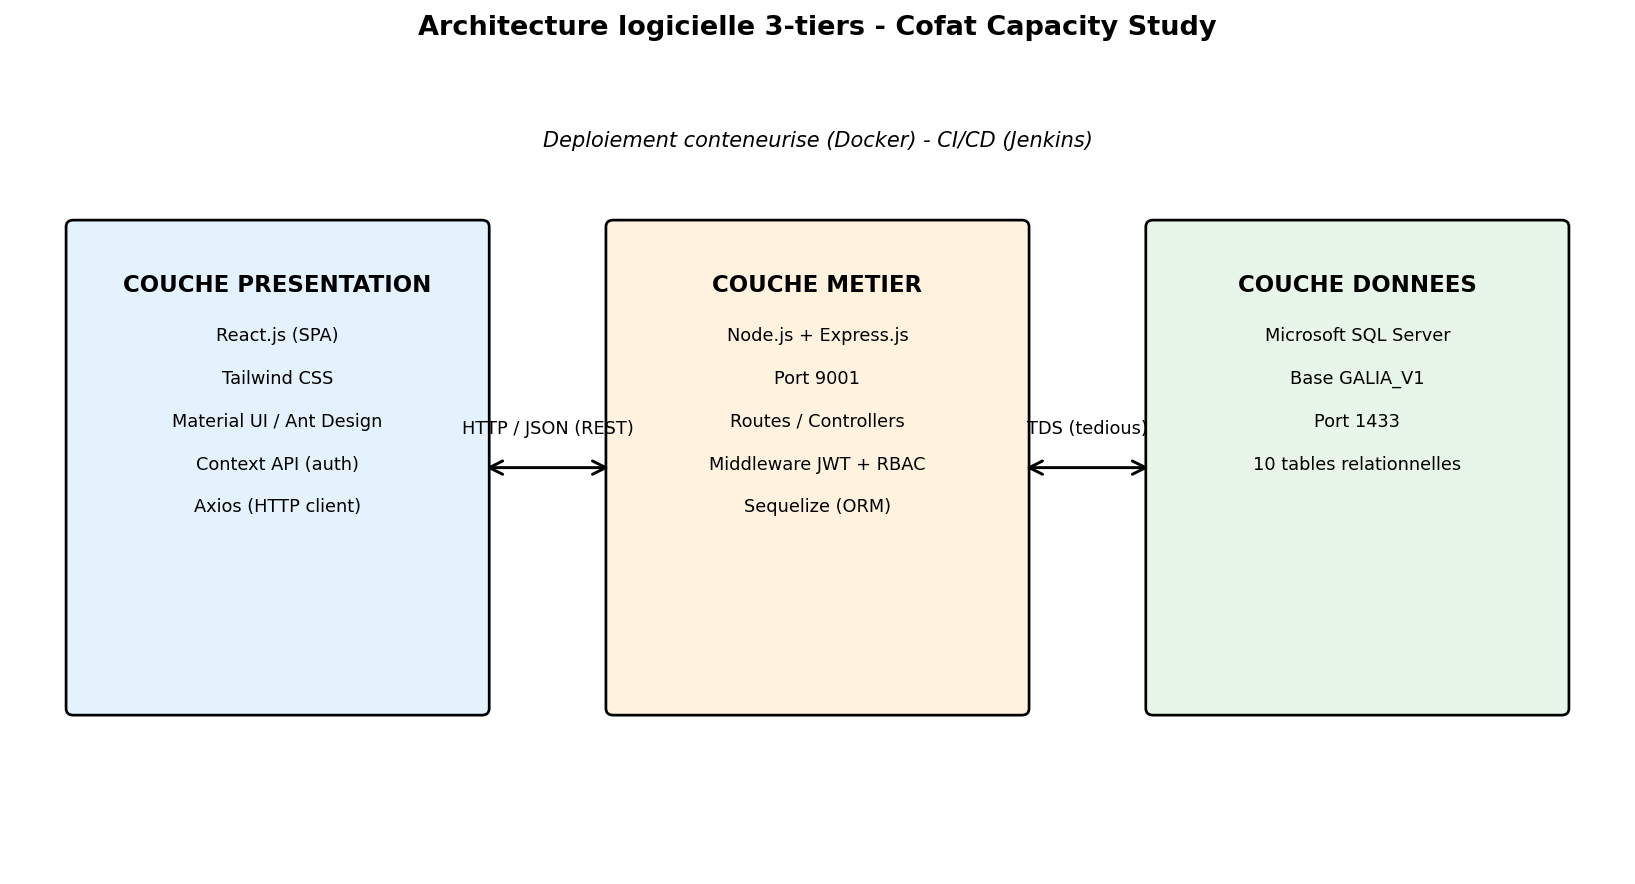
\includegraphics[width=0.85\textwidth]{img/architecture_logicielle.png}
    \caption{Architecture logicielle 3-tiers de l'application}
    \label{fig:arch_3tiers_ch3}
\end{figure}

\begin{figure}[H]
    \centering
    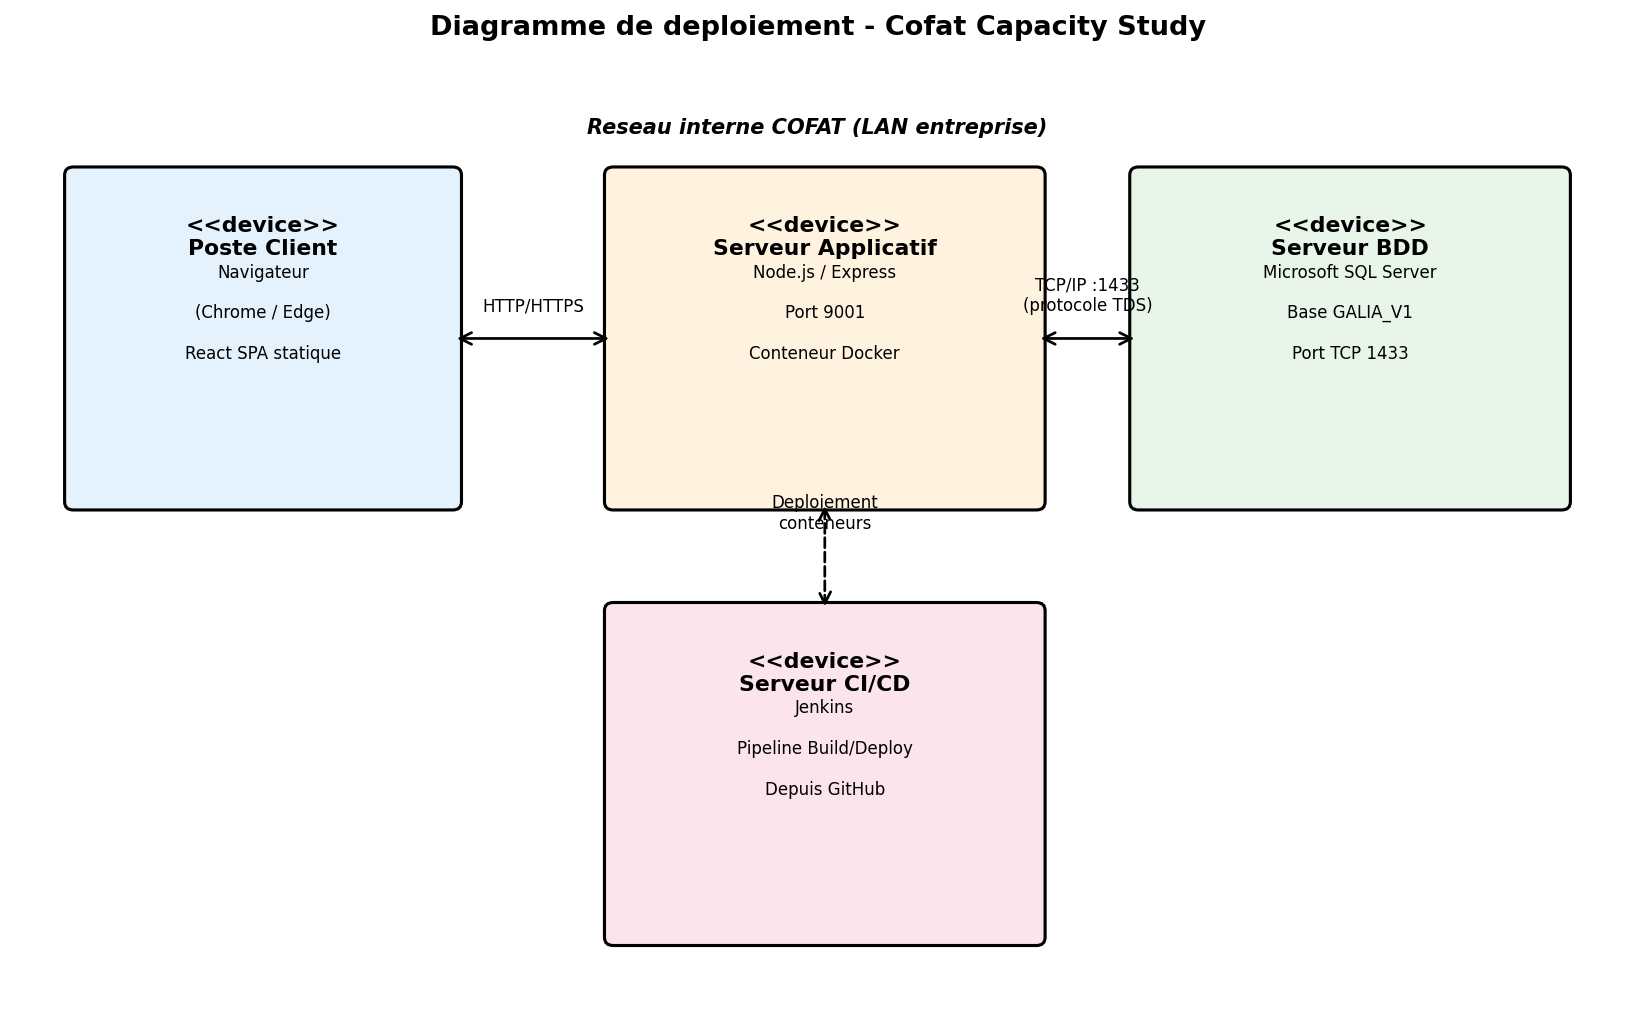
\includegraphics[width=0.85\textwidth]{img/diagramme_deploiement.png}
    \caption{Diagramme de déploiement réseau de Cofat Capacity Study}
    \label{fig:deploiement_ch3}
\end{figure}

\subsection{Spécification des besoins fonctionnels}
La page de Login est la porte d'entrée unique. Avant même de traiter les identifiants, le serveur applique un \textit{rate limiter} (bibliothèque \texttt{express-rate-limit}) qui bloque les adresses IP après 5 tentatives infructueuses, et une validation de schéma via \texttt{Joi}.

\begin{figure}[H]
    \centering
    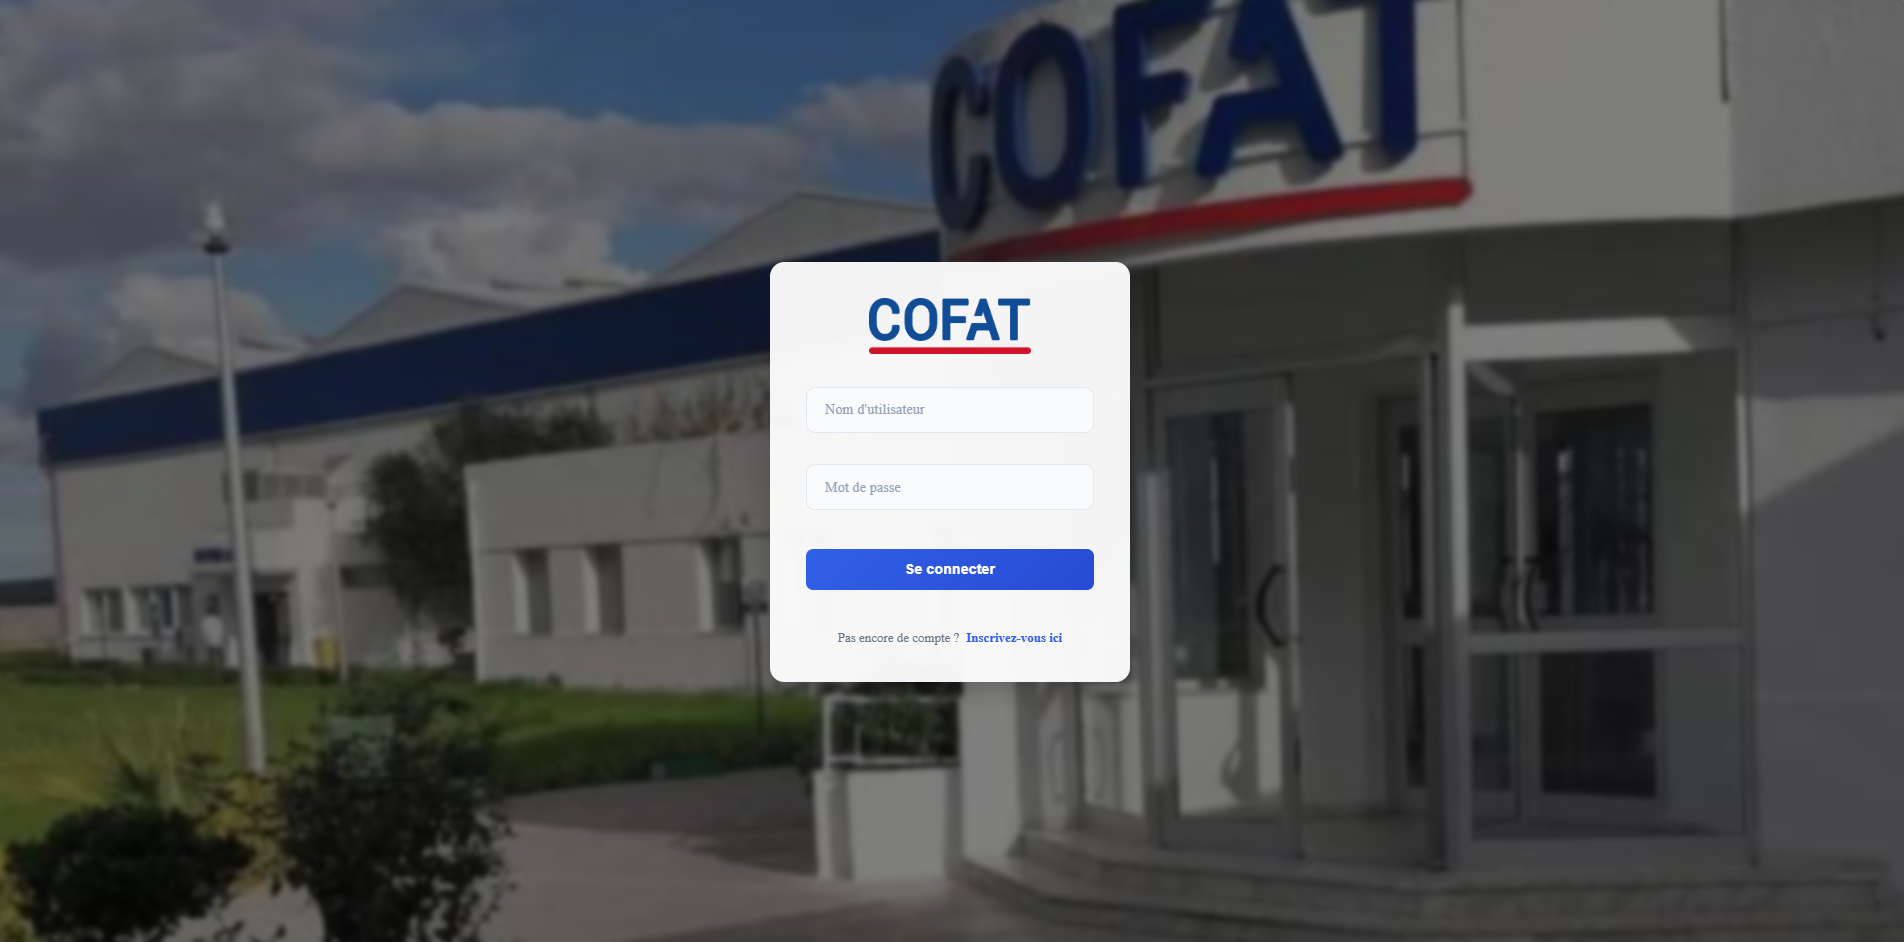
\includegraphics[width=0.75\textwidth]{img/auth_screen.png}
    \caption{Interface d'authentification de l'application}
    \label{fig:auth_screen_ch3}
\end{figure}

\subsection{Diagramme de classes}
La gestion des identités et du découpage multi-sites repose sur les modèles Sequelize \texttt{User} et \texttt{Site}. Le modèle \texttt{User} définit les trois rôles applicatifs (\texttt{admin}, \texttt{user}, \texttt{Achat}) et sécurise les mots de passe via un hachage bcrypt appliqué automatiquement avant chaque insertion en base de données.

\subsection{Diagrammes dynamiques}
Le diagramme de séquence de la Figure \ref{fig:seq_auth_ch3} détaille le processus d'authentification et de génération du cookie HttpOnly.

\begin{figure}[H]
    \centering
    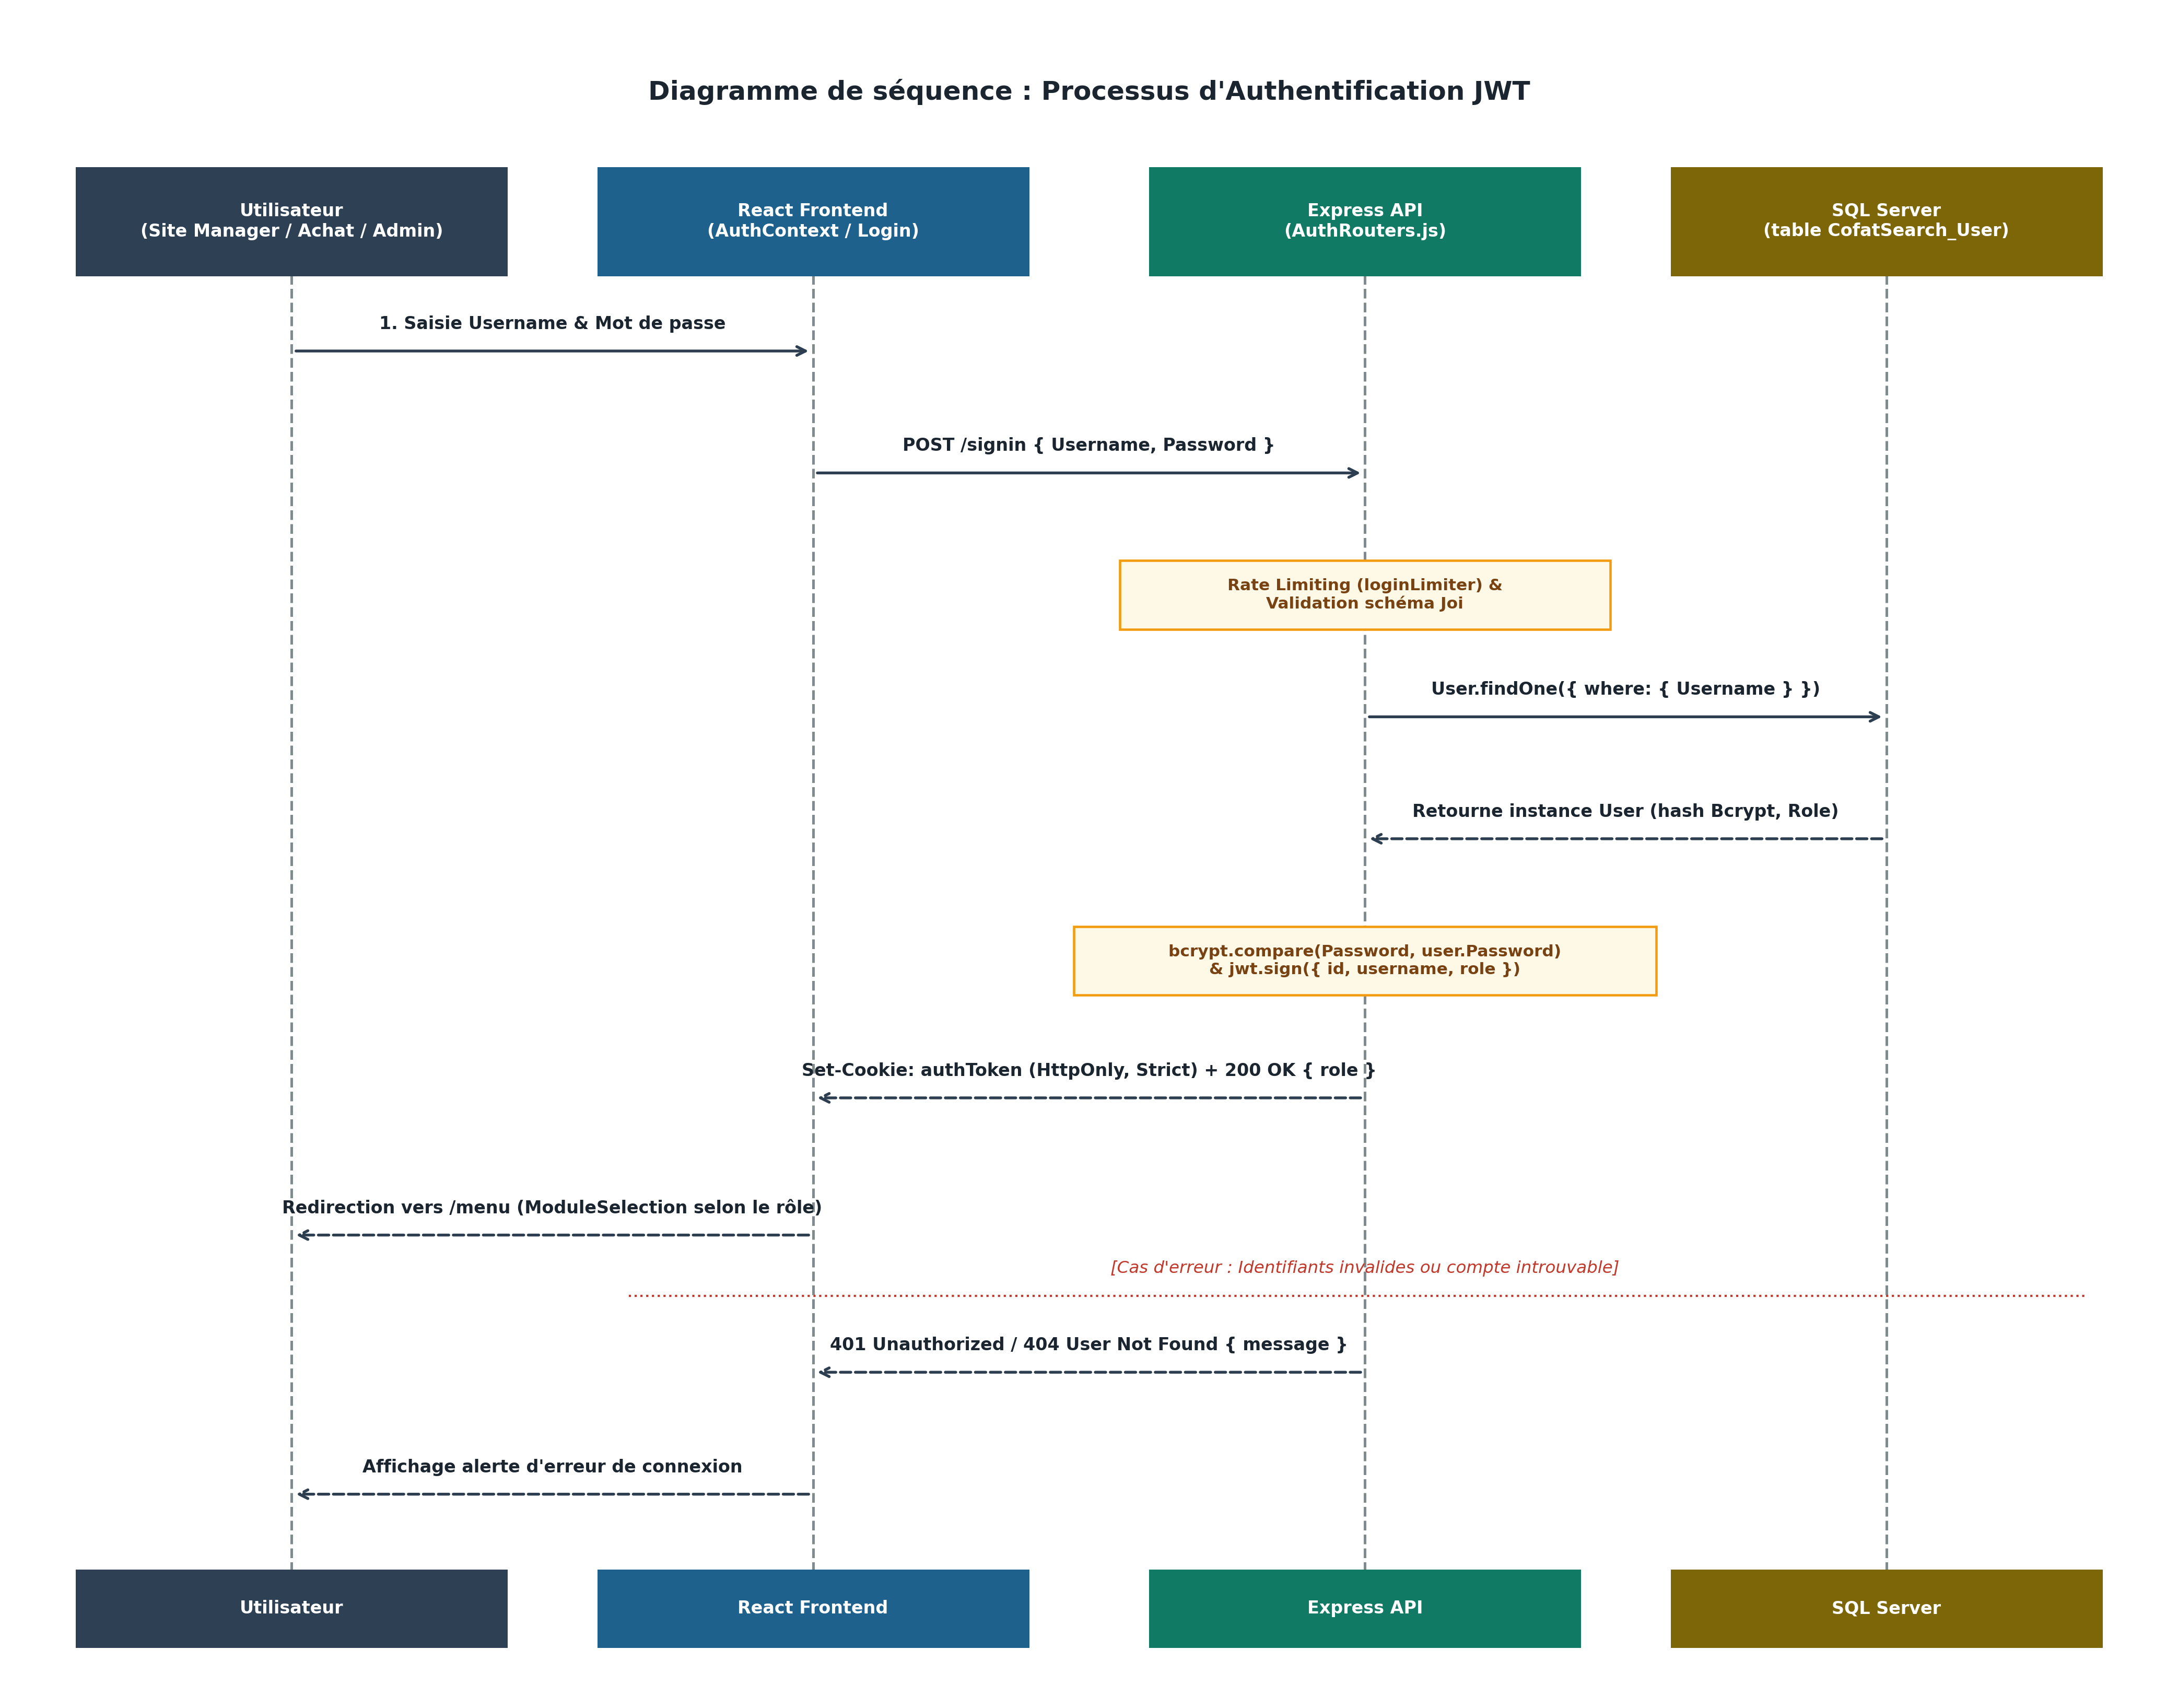
\includegraphics[width=0.85\textwidth]{img/sequence_auth.png}
    \caption{Diagramme de séquence du processus d'authentification JWT}
    \label{fig:seq_auth_ch3}
\end{figure}

\subsection{Réalisation}
Une fois authentifié en tant qu'Admin, l’utilisateur accède à son espace de pilotage central (Figures \ref{fig:admin_dash_ch3} et \ref{fig:home_nav_ch3}).

\begin{figure}[H]
    \centering
    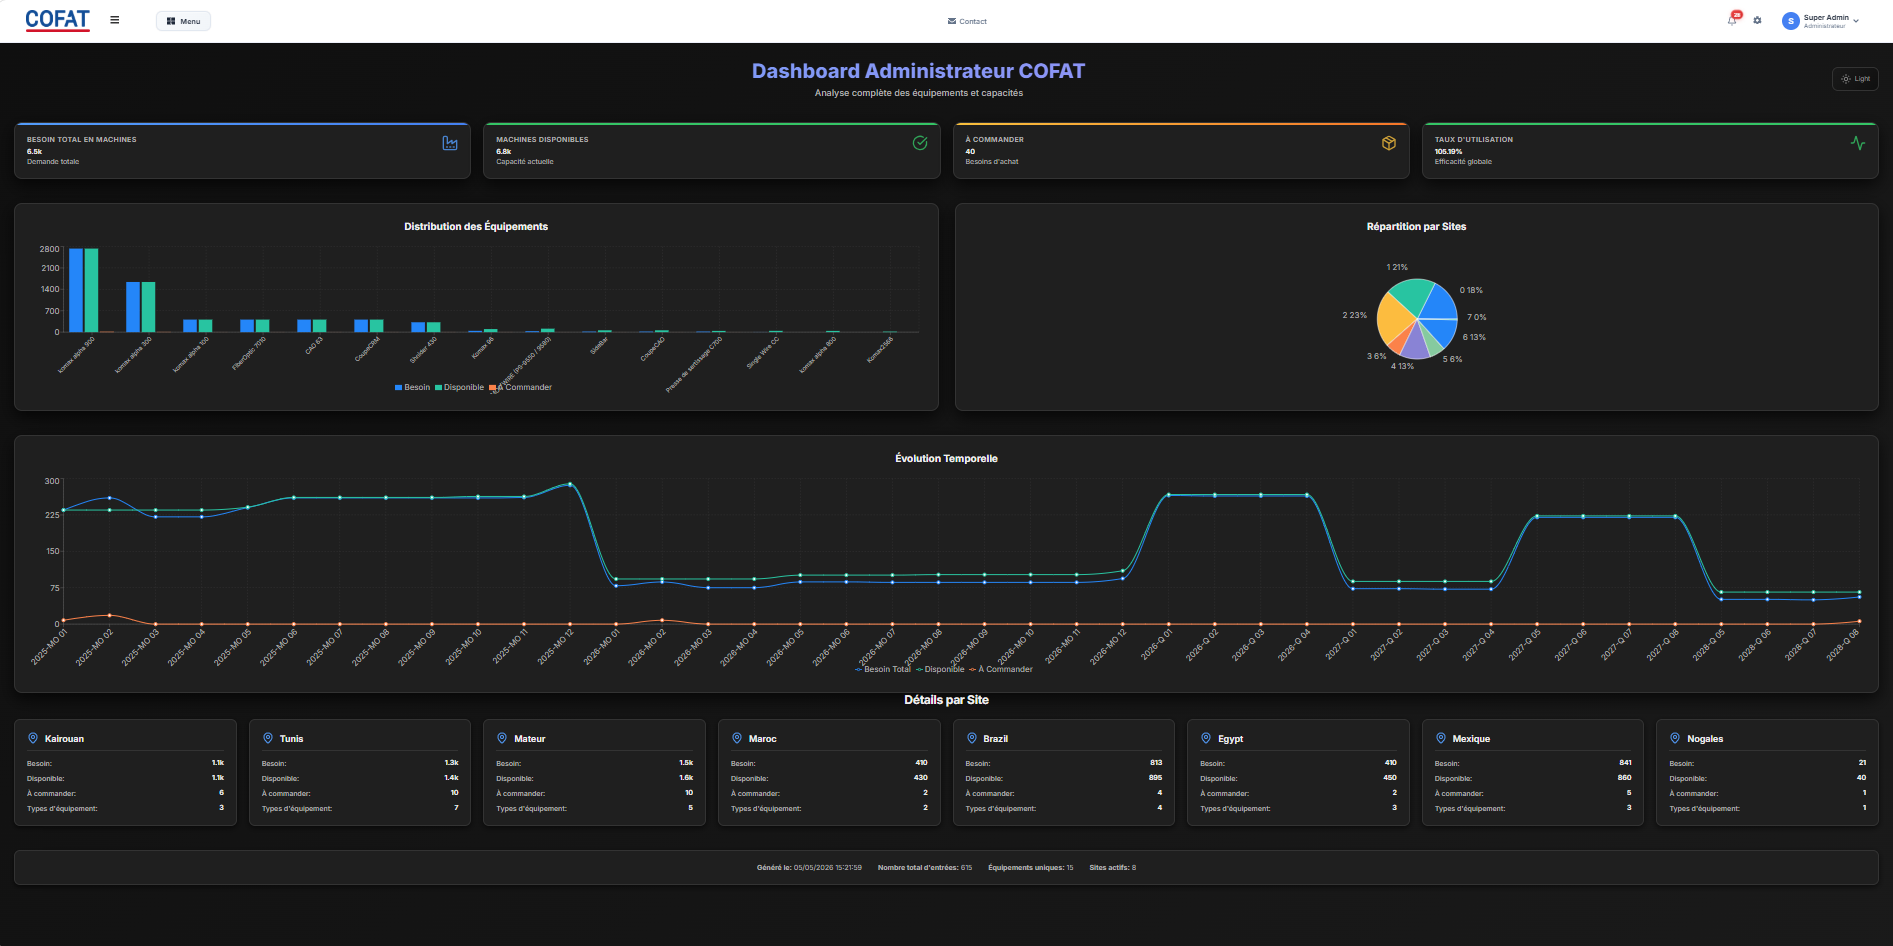
\includegraphics[width=0.9\textwidth]{img/admin_dashboard.png}
    \caption{Tableau de bord de l'Administrateur}
    \label{fig:admin_dash_ch3}
\end{figure}

\begin{figure}[H]
    \centering
    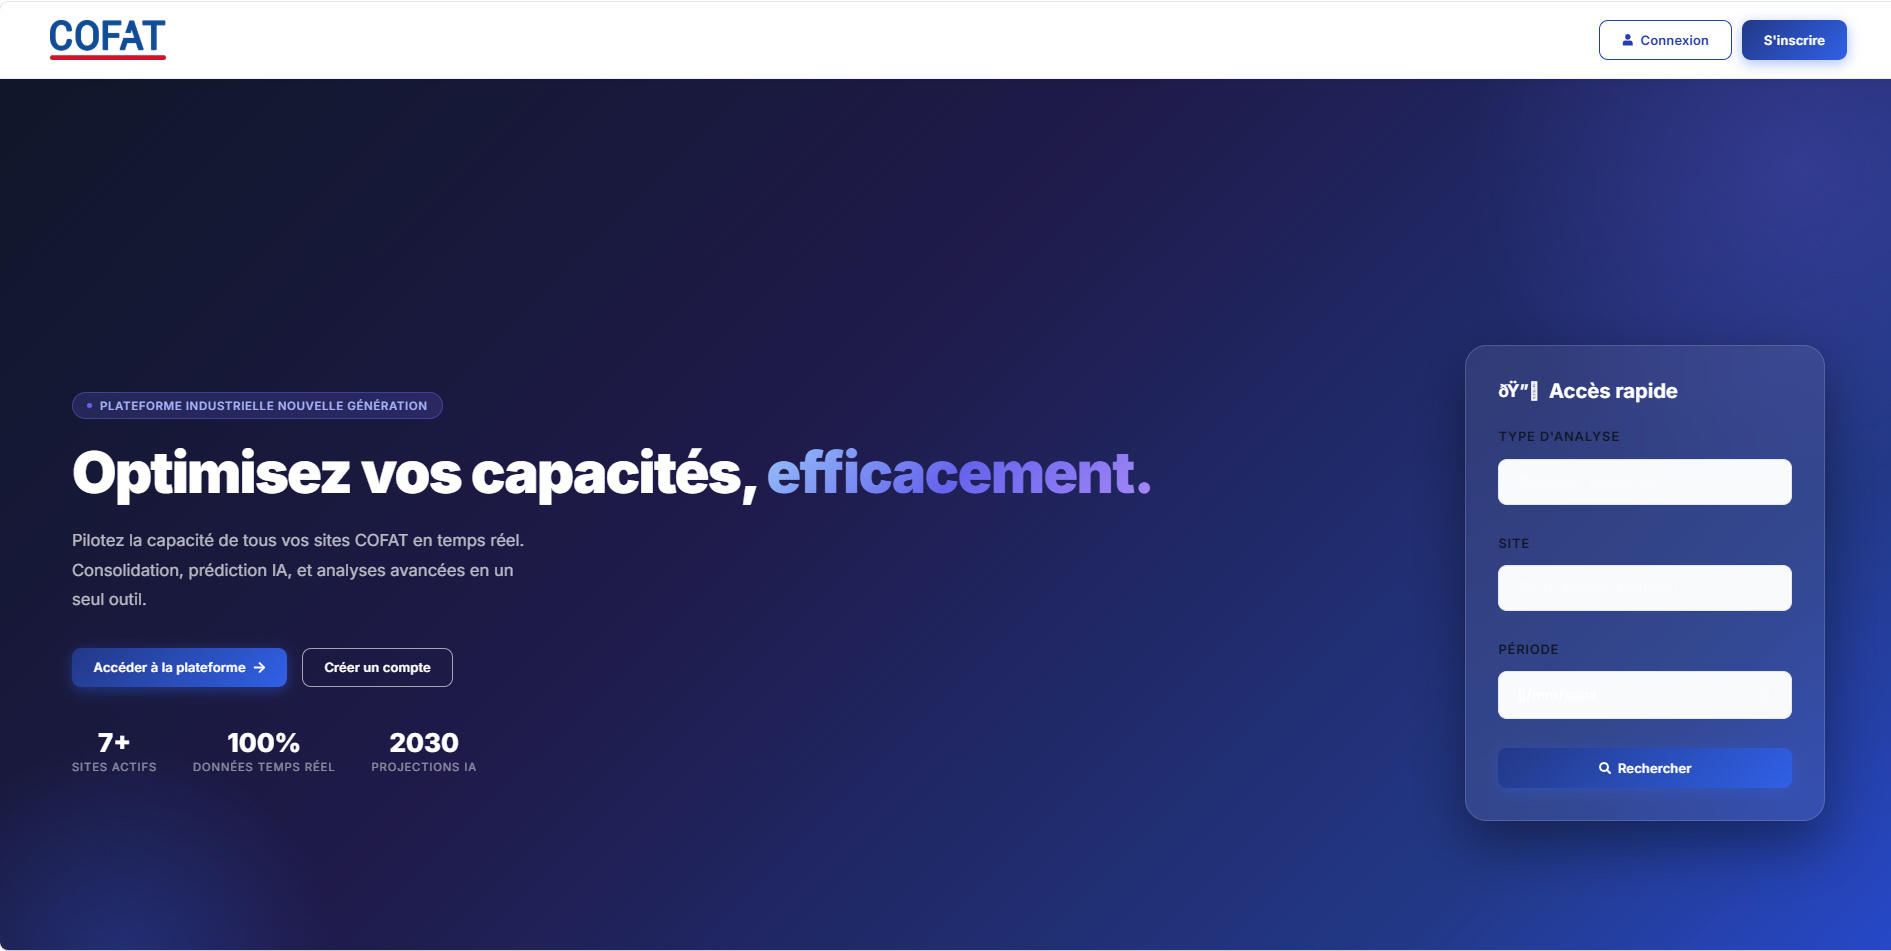
\includegraphics[width=0.9\textwidth]{img/home_page.png}
    \caption{Menu de navigation principal (Home Page)}
    \label{fig:home_nav_ch3}
\end{figure}

\subsubsection{Validation et recette du sprint 1}
Le Tableau \ref{tab:recette_s1_ch3} présente le cahier de recette validé avec le Product Owner.

\begin{table}[h]
\centering
\begin{tabular}{|p{1.5cm}|p{4.5cm}|p{5cm}|p{2.5cm}|}
\hline
\textbf{ID Test} & \textbf{Cas de test exécuté} & \textbf{Résultat attendu} & \textbf{Statut} \\ \hline
TEST-01 & Connexion avec identifiants valides & Token JWT généré, cookie HttpOnly posé, redirection Dashboard & \textbf{VALIDÉ} \\ \hline
TEST-02 & Connexion avec mot de passe erroné & Erreur 401 "Identifiants invalides", aucun token émis & \textbf{VALIDÉ} \\ \hline
TEST-03 & Accès route `/api/dashboard/admin` sans token & Erreur 401 "Accès refusé : Jeton absent" & \textbf{VALIDÉ} \\ \hline
TEST-04 & Accès administration par un rôle non-admin & Erreur 403 "Accès refusé. Réservé aux administrateurs" & \textbf{VALIDÉ} \\ \hline
TEST-05 & Consultation du référentiel des 10 sites & Récupération JSON des 10 sites (\texttt{/api/sites}) & \textbf{VALIDÉ} \\ \hline
\end{tabular}
\caption{Cahier de recette fonctionnelle du Sprint 1}
\label{tab:recette_s1_ch3}
\end{table}


\section{Sprint 2 : Module de planification locale et import Excel}

\subsection{Objectifs du sprint 2}
Le Sprint 2 visait à fournir aux Site Managers d'usine l'autonomie nécessaire pour saisir, importer via Excel et analyser leurs capacités locales (Équipements, Espaces et Ressources Humaines).

\subsection{Backlog du sprint 2}
Le Tableau \ref{tab:backlog_sprint2} détaille le backlog du Sprint 2 centré sur les modules de planification locale et le moteur d'importation Excel.

\begin{table}[H]
\centering
\begin{tabular}{|c|p{9.2cm}|c|c|}
\hline
\textbf{Id} & \textbf{Fonctionnalités (User Story)} & \textbf{Priorité} & \textbf{Estimation (Jours)} \\ \hline
12 & En tant que Site Manager, je veux sélectionner mon usine et l'année d'exercice afin de charger les données capacitaires associées. & 1 & 2 \\ \hline
13 & En tant que Site Manager, je veux saisir manuellement le besoin capacitaire machine (\texttt{machineNeed}) par équipement et par mois. & 1 & 3 \\ \hline
14 & En tant que Site Manager, je veux renseigner le parc de machines physiques disponibles (\texttt{availableMachine}) dans mon atelier. & 1 & 2 \\ \hline
15 & En tant que Site Manager, je veux que le système calcule automatiquement le taux de charge capacitaire ($Load$) en pourcentage. & 1 & 2 \\ \hline
16 & En tant que Site Manager, je veux que le système calcule automatiquement le nombre de machines manquantes à commander (\texttt{toOrder}). & 1 & 2 \\ \hline
17 & En tant que Site Manager, je veux visualiser des codes couleurs d'alerte selon la criticité du taux de charge machine. & 1 & 2 \\ \hline
18 & En tant que Site Manager, je veux téléverser des fichiers Excel (.xlsx) pour importer massivement les prévisions de charge. & 1 & 3 \\ \hline
19 & En tant que Site Manager, je veux que le serveur analyse et valide la structure des fichiers Excel importés avec Multer et SheetJS. & 1 & 3 \\ \hline
20 & En tant que Site Manager, je veux que les données Excel soient injectées en masse dans SQL Server via \texttt{bulkCreate} sans doublons. & 1 & 3 \\ \hline
21 & En tant que Site Manager, je veux recevoir un rapport explicite en cas d'erreur de format ou de données dans le fichier Excel. & 2 & 2 \\ \hline
22 & En tant que Site Manager, je veux modéliser l'occupation des surfaces d'atelier en $m^2$ par catégorie de zone industrielle. & 1 & 3 \\ \hline
23 & En tant que Site Manager, je veux comparer la surface occupée à la surface totale bâtie de l'usine pour évaluer la réserve spatiale. & 1 & 2 \\ \hline
24 & En tant que Site Manager, je veux planifier les effectifs de main-d'œuvre directe (MOD) par projet client sur un horizon de 3 ans. & 1 & 3 \\ \hline
25 & En tant que Site Manager, je veux planifier les effectifs de main-d'œuvre indirecte (MOI) et des services support de mon site. & 1 & 2 \\ \hline
26 & En tant que Site Manager, je veux consulter les courbes prévisionnelles d'évolution des effectifs pour anticiper les recrutements. & 2 & 2 \\ \hline
27 & En tant que Site Manager, je veux consulter les graphiques de synthèse capacitaire locale pour préparer les revues de production. & 2 & 1 \\ \hline
\end{tabular}
\caption{Backlog du Sprint 2}
\label{tab:backlog_sprint2}
\end{table}

\subsection{Spécification des besoins fonctionnels}
Le module Équipements permet de suivre l'état de saturation du parc machine et de calculer automatiquement le taux de charge $Load = (machineNeed / availableMachine) \times 100$. Un code couleur visuel (conditional formatting) alerte le responsable (Vert $\le 80\%$, Orange $80\% < Load \le 100\%$, Rouge $> 100\%$).

\begin{figure}[H]
    \centering
    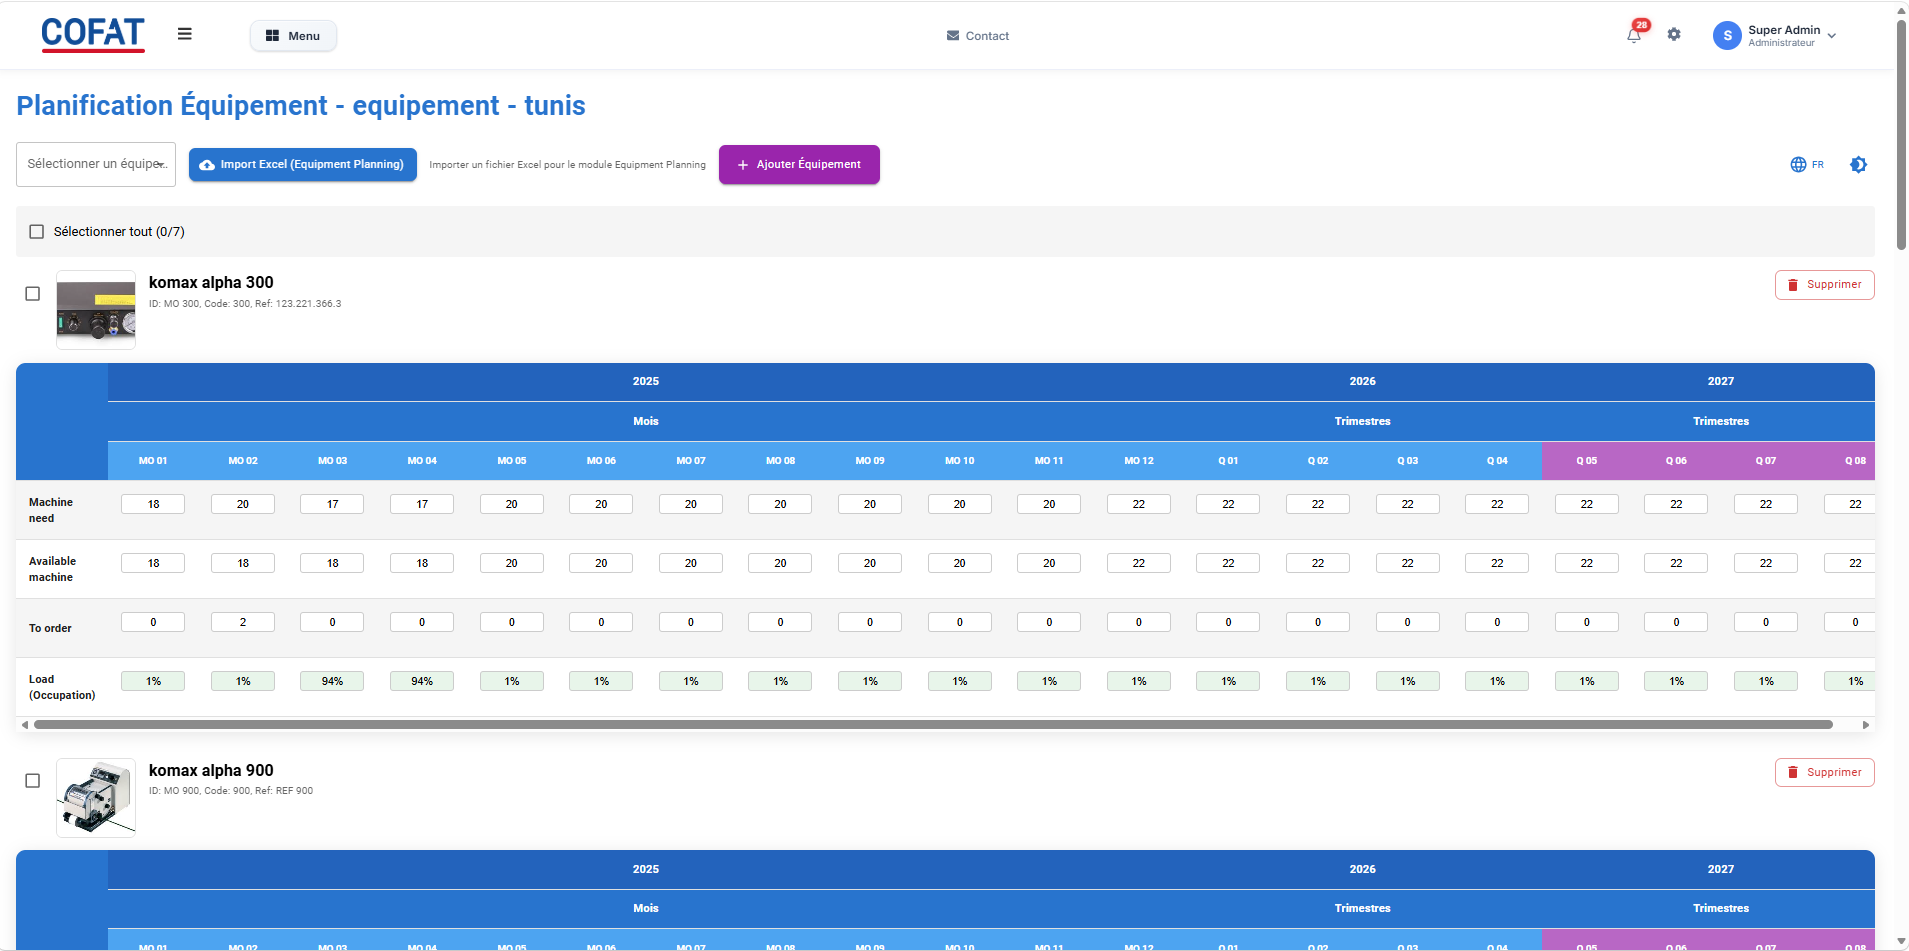
\includegraphics[width=0.9\textwidth]{img/planification_equipement.png}
    \caption{Interface de planification locale des équipements}
    \label{fig:equip_plan_ch3}
\end{figure}

Le module Espaces gère l'occupation des surfaces au sol ($m^2$) par zone de production (Magasin, Cutting, Assembly, Shipping).

\begin{figure}[H]
    \centering
    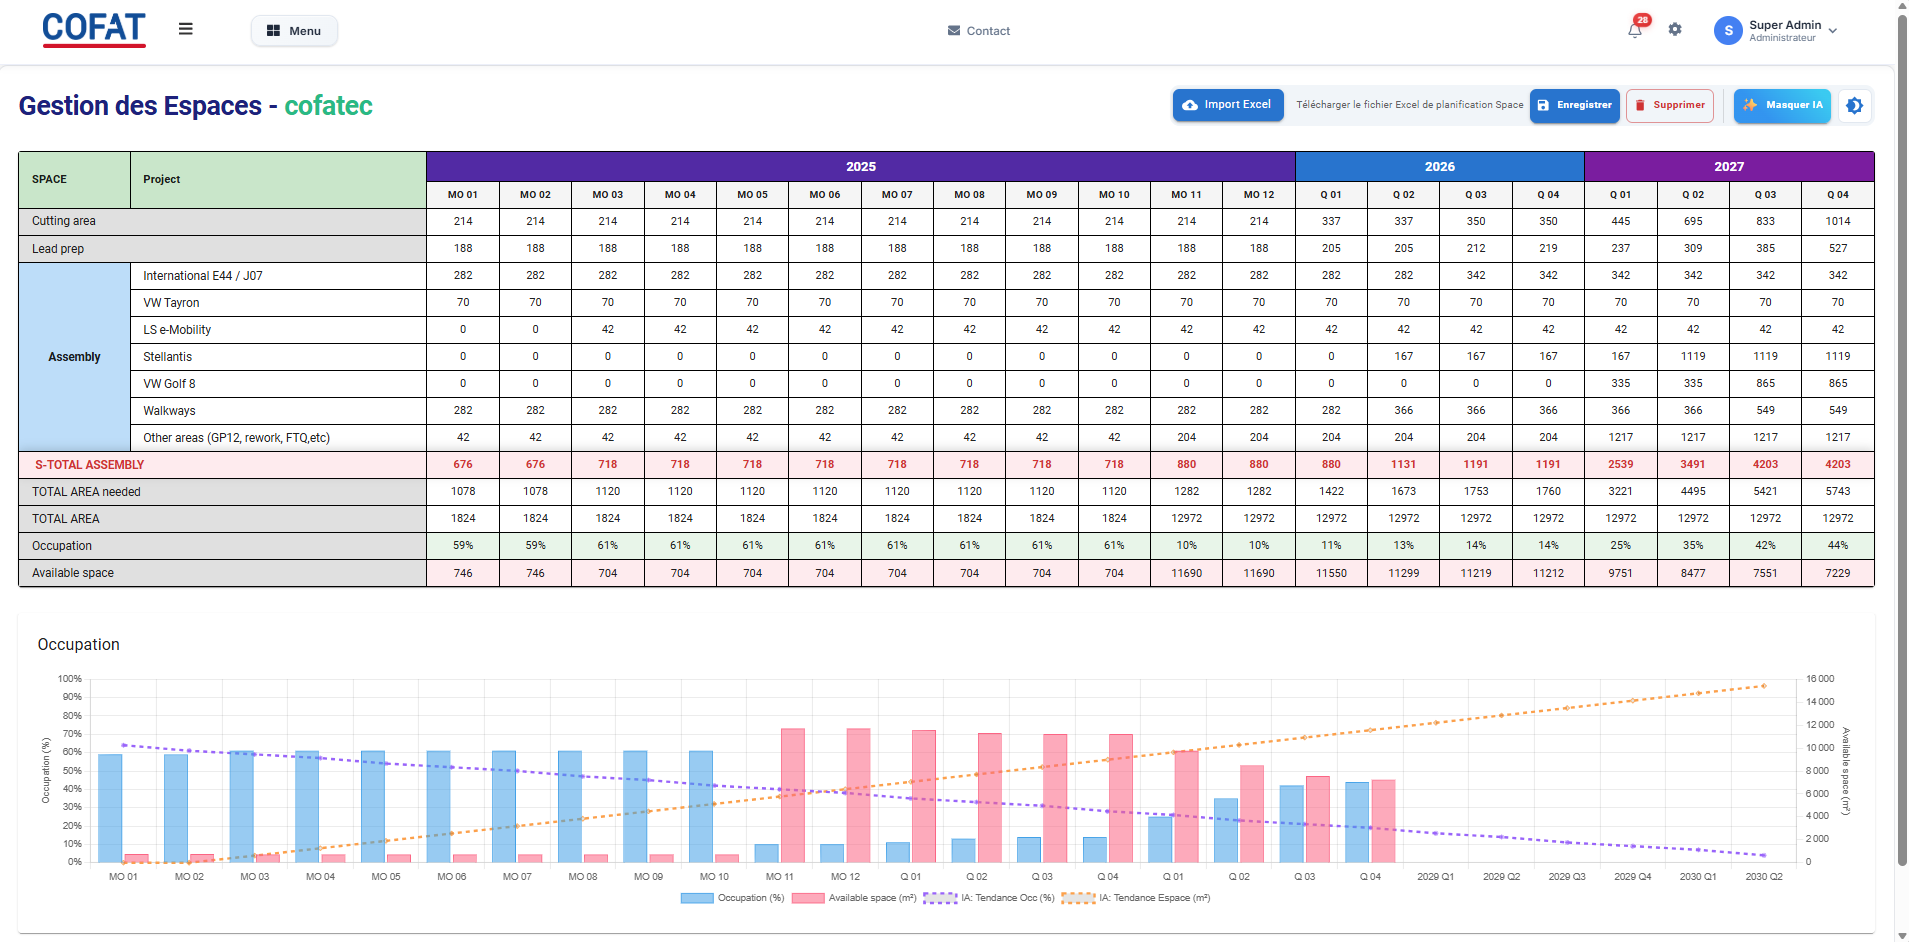
\includegraphics[width=0.9\textwidth]{img/gestion_espaces.png}
    \caption{Tableau de gestion des surfaces par zone de production}
    \label{fig:spaces_plan_ch3}
\end{figure}

\begin{figure}[H]
    \centering
    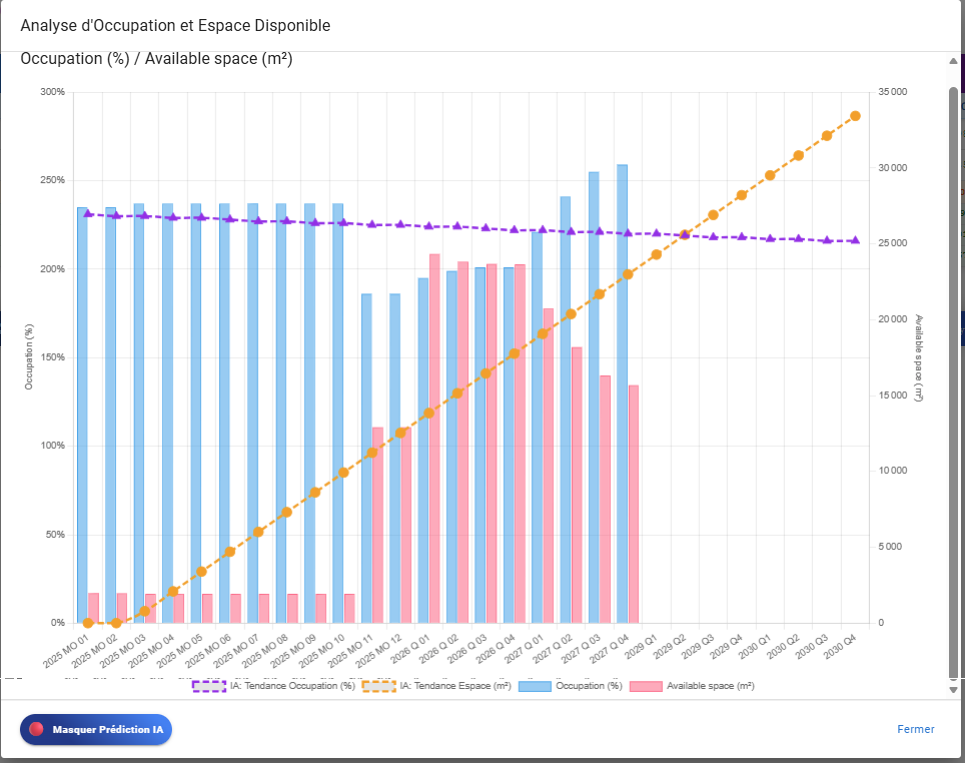
\includegraphics[width=0.85\textwidth]{img/dashboard_espaces.png}
    \caption{Tableau de bord visuel : Taux d'occupation global du site}
    \label{fig:spaces_dash_ch3}
\end{figure}

Le module RH projette les besoins en effectifs (directs et indirects) sur une matrice temporelle de 3 ans (12 mois + 8 trimestres).

\begin{figure}[H]
    \centering
    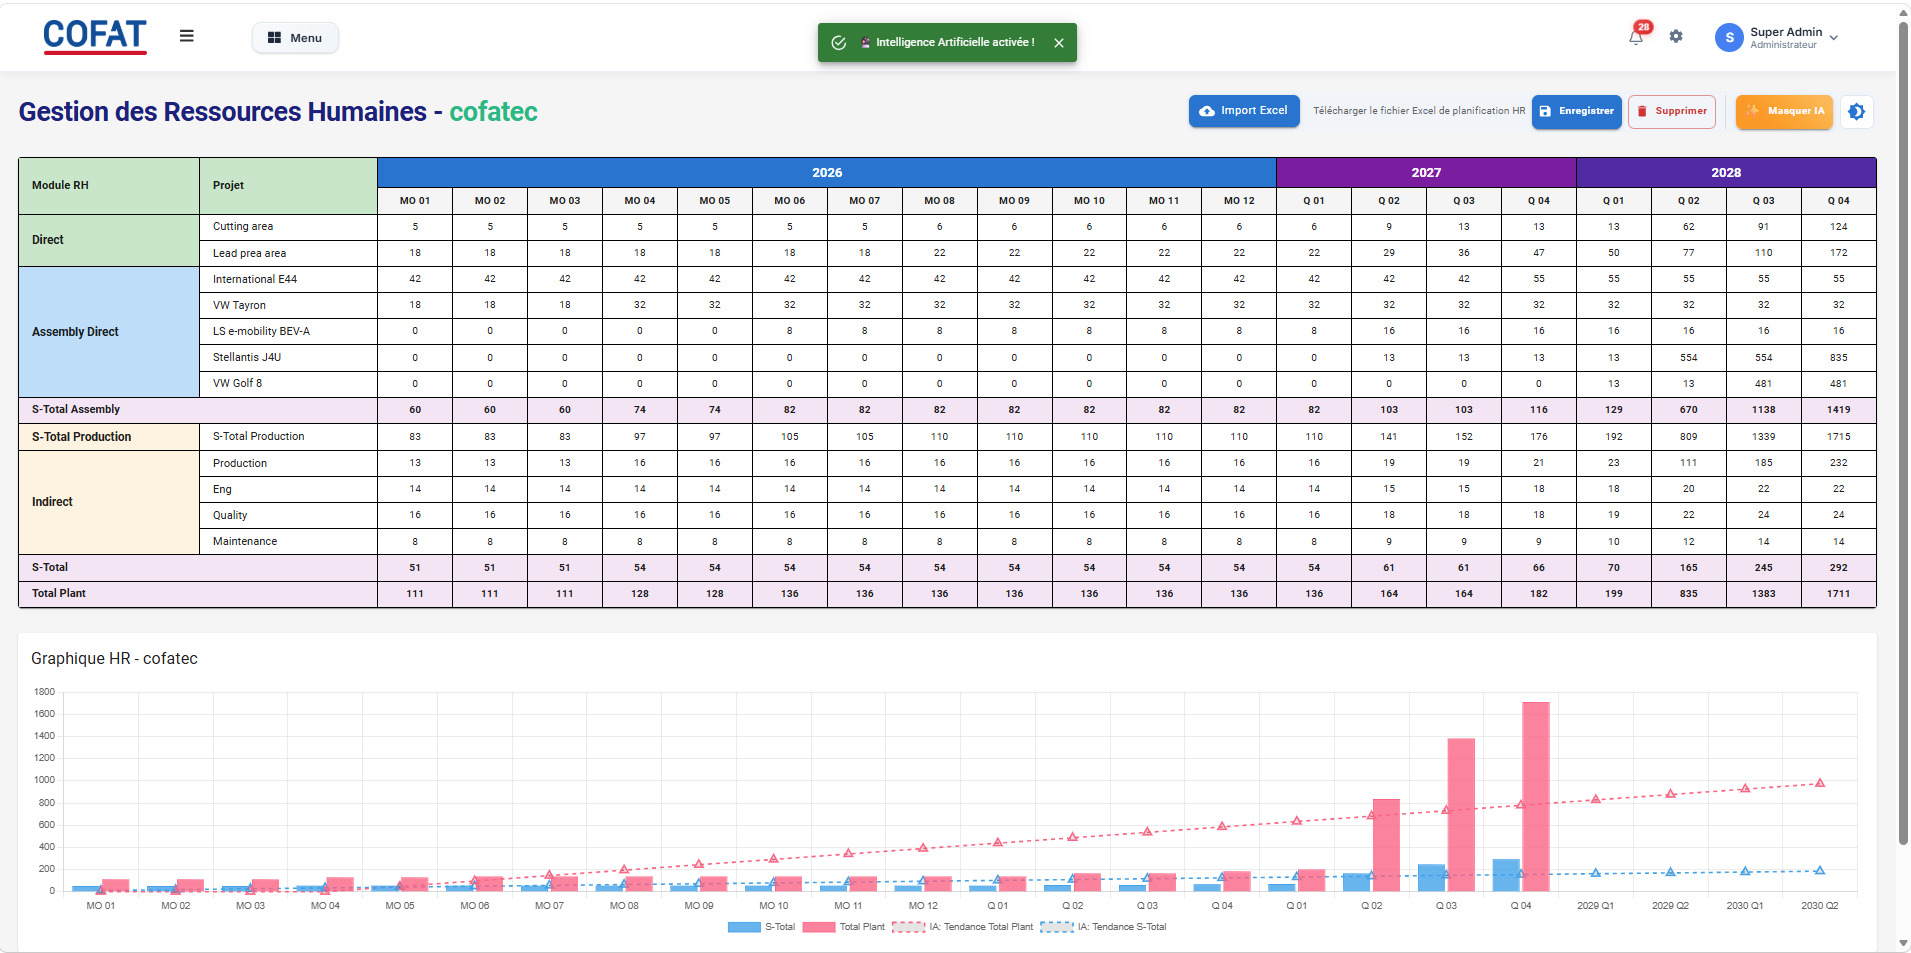
\includegraphics[width=0.9\textwidth]{img/planification_rh.png}
    \caption{Interface de planification temporelle des Ressources Humaines}
    \label{fig:hr_plan_ch3}
\end{figure}

\subsection{Diagramme de classes}
Les entités métier associées au Sprint 2 sont \texttt{Equipment}, \texttt{EquipmentPlanning}, \texttt{Spaces} et \texttt{HR}.

\subsection{Diagrammes dynamiques}
Le pipeline d'importation Excel repose sur un traitement multipart intercepté par \texttt{multer}, parsé par \texttt{xlsx} et inséré en BDD via Sequelize \texttt{bulkCreate}.

\begin{figure}[H]
    \centering
    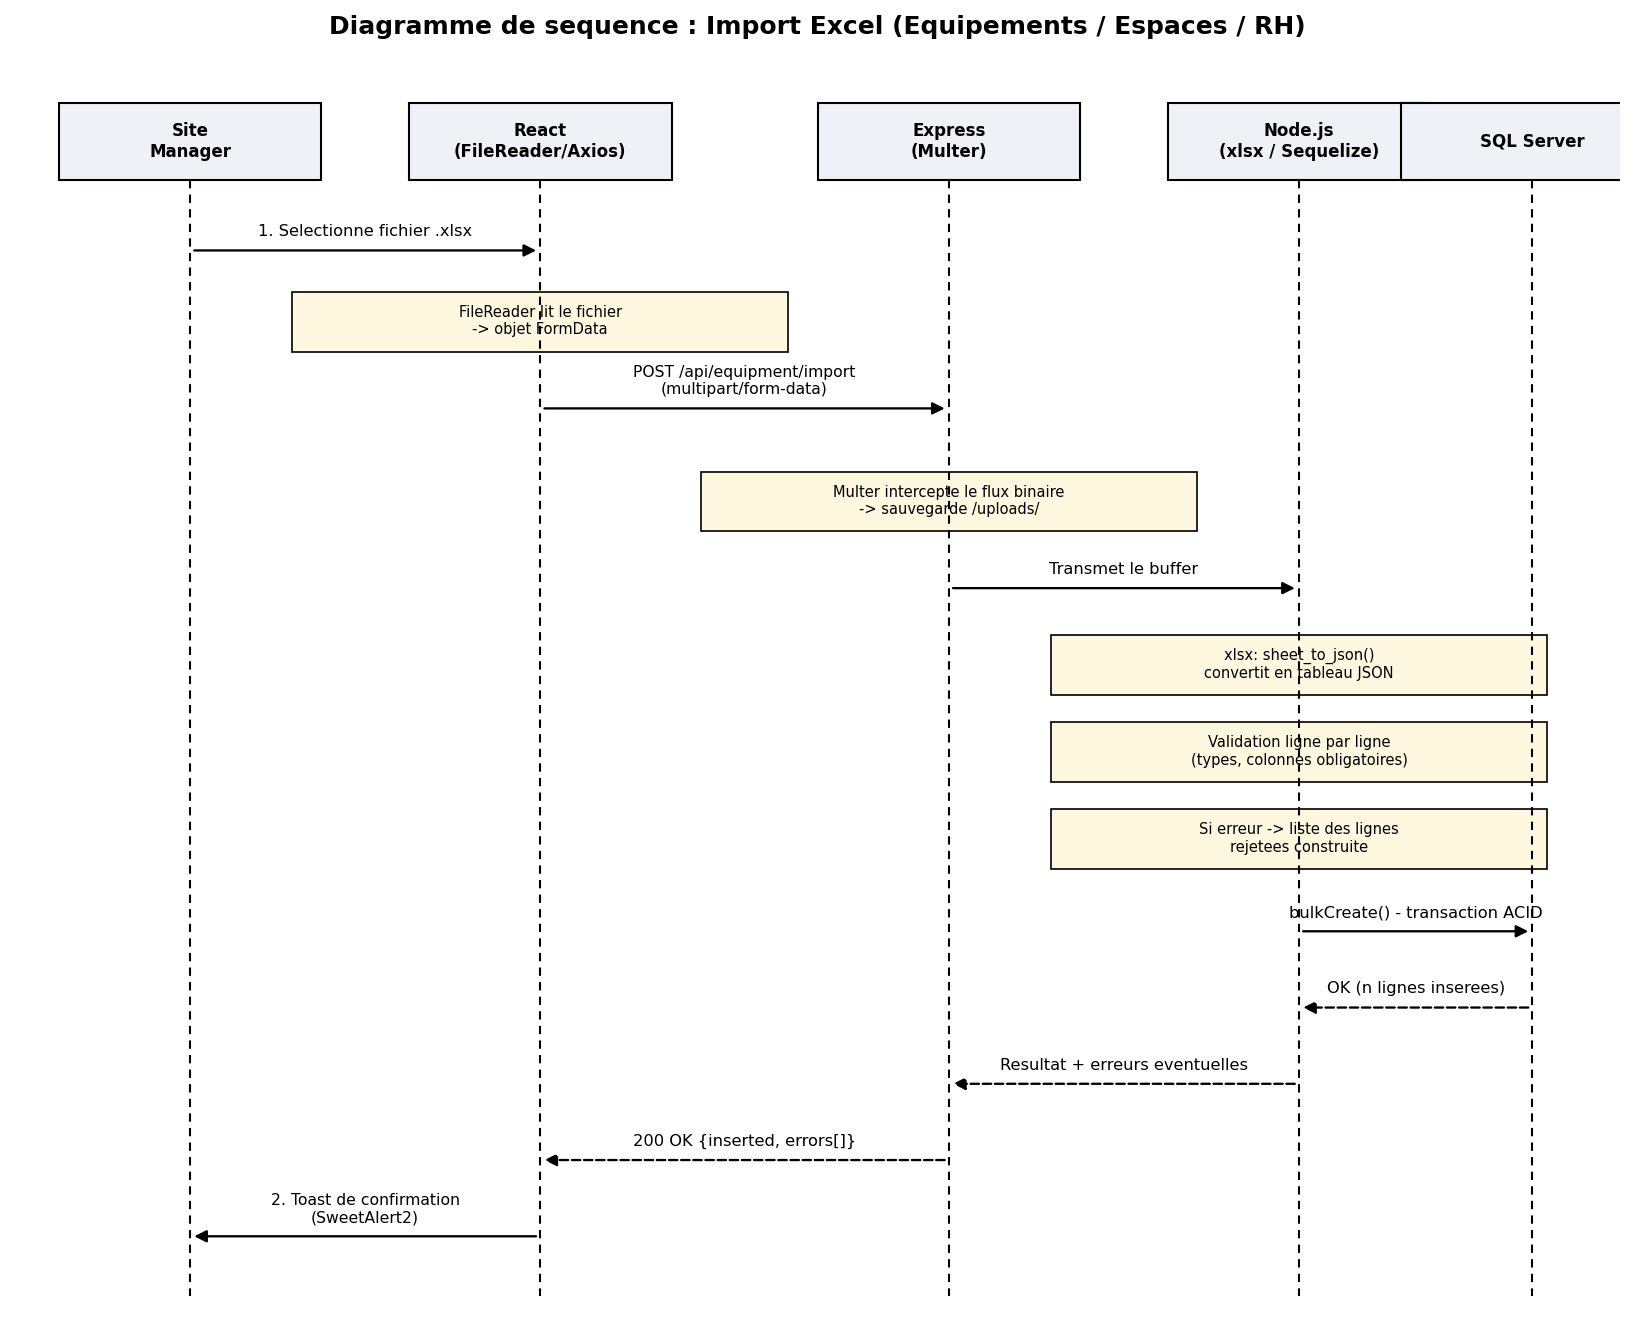
\includegraphics[width=0.85\textwidth]{img/sequence_import_excel.png}
    \caption{Diagramme de séquence du processus d'import Excel}
    \label{fig:seq_excel_ch3}
\end{figure}



\subsection{Réalisation}
Les vues de planification locale permettent aux Site Managers d'éditer ou d'importer directement leurs données de production.

\subsubsection{Validation et recette du sprint 2}
Tous les cas d'usage de la planification locale et de l'importation Excel ont été testés et validés lors de la Sprint Review du Sprint 2.

\section*{Conclusion}
Au terme de cette Release 1 (Sprints 1 et 2), le socle applicatif, la gestion des accès et les modules de planification locale des usines sont pleinement opérationnels.
